%%%%%%%%%%%%%%%%%%%%%%%%%%%%%%%%%%%%%%%%%%%%%%%%%%%%%%%%%%%%%%%%%%%%%%%%
% TFG: Vigilancia Tecnológica y Minería de Opiniones en RRSS
% Escuela Técnica Superior de Ingenierías Informática y de Telecomunicación
% Realizado por: Miguel Keane Cañizares
% Contacto: miguekeca@correo.ugr.es 
%%%%%%%%%%%%%%%%%%%%%%%%%%%%%%%%%%%%%%%%%%%%%%%%%%%%%%%%%%%%%%%%%%%%%%%%

\chapter{Implementación}

La mayor parte del proceso de implementación estará enfocado a la creación de los scripts que sean necesarios. Primero implementaremos un programa al que llamaremos \textit{ladrón de tweets} el cual será el encargado de obtener la información de Twitter, crear una base de datos MongoDB y almacernar los datos obtenidos en la misma. 


\subsection{Ladrón de Tweets}

Este código hará uso de las librerías de Tweepy para acceder a la API de Twitter y las librerías de MongoDB para almacenar la información.

\begin{figure}[h]
	\centering
	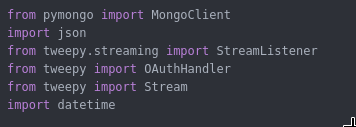
\includegraphics[scale=.6]{imagenes/include-ladron.png}
	\caption{Librerías de ladrón de tweets}
	\label{fig:include-ladron}
\end{figure}


Lo siguiente que hacemos es crear y conectarnos a la base de datos MongoDB, en la cuál almacenaremos toda la información que posteriormente descarguemos. 

\begin{figure}[h]
	\centering
	\includegraphics[scale=1.5]{imagenes/crearMongodb-ladron.png}
	\caption{Inicialización de base de datos MongoDB}
	\label{fig:crear-mongodb}
\end{figure}


Posteriormente es necesario declarar las variables que usaremos al usar la API de Twitter. El idioma que buscará, las claves de acceso y las palabras claves que deseamos descargar. 

\begin{figure}[h]
	\centering
	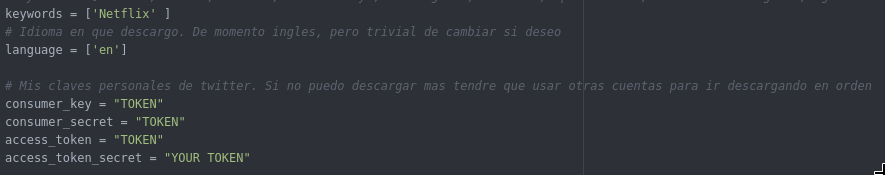
\includegraphics[scale=.4]{imagenes/token-ladron.png}
	\caption{Declaración de variables de acceso, búsqueda e idioma}
	\label{fig:token-ladron}
\end{figure}


Llegado este punto, deberemos hacer la conexión con la API de Twitter mediante las funcionalidades de Tweepy, usando las variables previamente declaradas. Con la función Stream, lo que hacemos es ponerlo en modo escucha, es decir, accederemos a los tweets que sean escritos en el tiempo de ejecución serán los que descarguemos. Debemos incluir el modo \textit{$tweet\_mode$=extended} el cual es necesario porque sino se usa solo se descargarán los primeros 140 caracteres del tweet, añadiendo información incompleta y por lo tanto desechable en la base de datos. 

\begin{figure}[h]
	\centering
	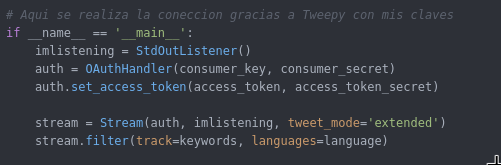
\includegraphics[scale=.5]{imagenes/inicio-sesion-ladron.png}
	\caption{Inicio de sesión en la API de Twitter}
	\label{fig:inicio-sesion-ladron}
\end{figure}


En la función \textit{StdOutListener()} tendremos la parte clave del script, en donde extraeremos la información del tweet y la almacenaremos en MongoDB. Al principio del código evitaremos descargar los Retweets, ya que por experiencia, estos Retweets lo que hacen es ensuciar la base de datos, puesto que si una persona con gran influencia en redes publica un tweet que es compartido por mucha gente, no aporta nueva información sino que almacena cientos o miles de veces la misma información, invalidando en parte los resultados de su posterior análisis. 

 
 \begin{figure}[H]
 	\centering
 	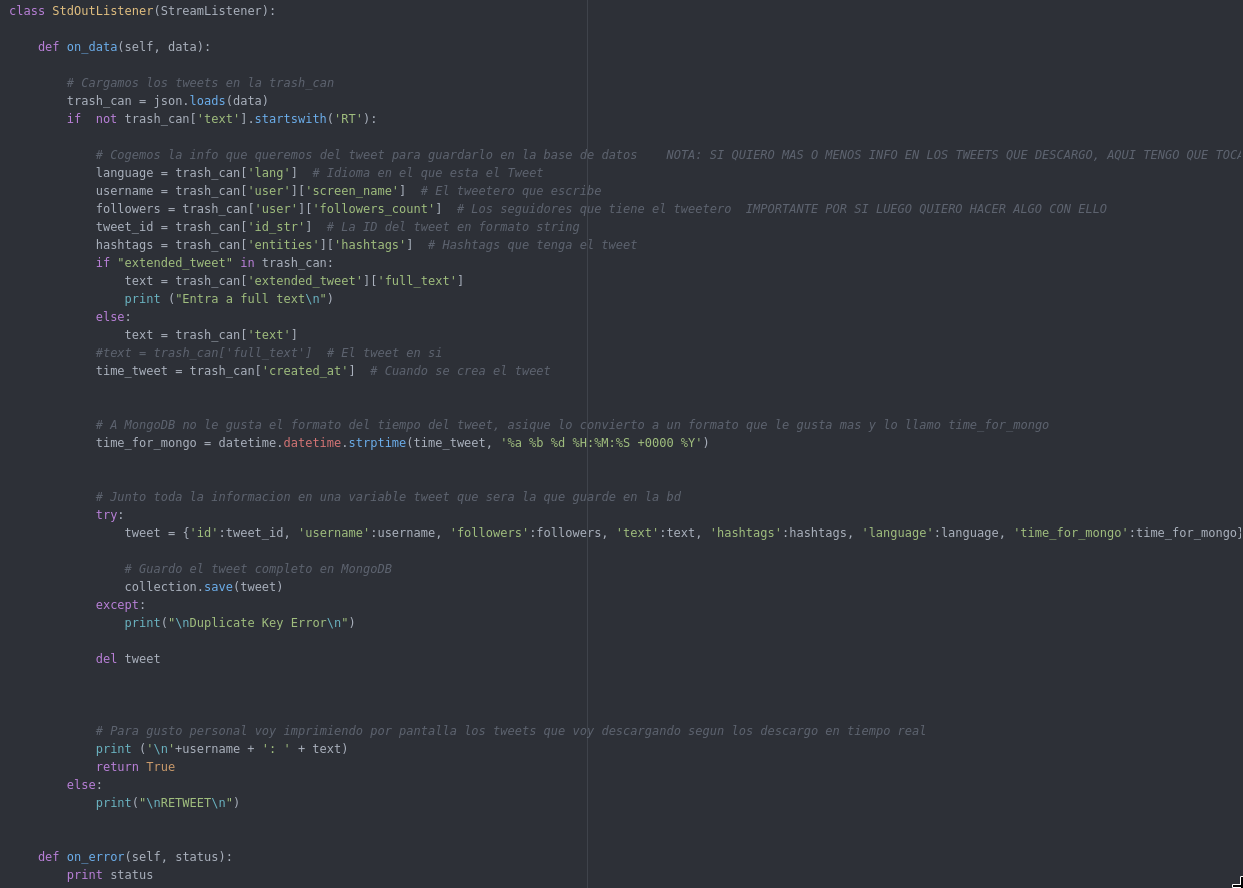
\includegraphics[scale=.35]{imagenes/codigo-ladron.png}
 	\caption{Función de captura y almacenamiento de tweets}
 	\label{fig:codigo-ladron}
 \end{figure}
















\subsection{Análisis Sentimientos}


Una vez existe una base de datos MongoDB hay que enviarla a analizar a MeaningCloud haciendo uso de su API. Luego de analizarla, obtendremos una información que será almacenada por partida doble, para facilitar la reutilización de la misma. Crearemos una colección diferente dentro de la base de datos MongoDB ya existente, a la que denominaremos \textit{concepts} y a la par se creará un archivo CSV en el cual almacenaremos toda la información para facilitar su posterior análisis. 

\begin{figure}[H]
	\centering
	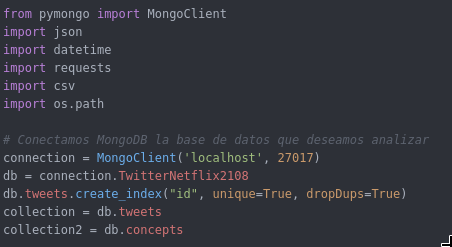
\includegraphics[scale=.35]{imagenes/include-analisis.png}
	\caption{Librerías utilizadas y declaración de la BD y creación de la nueva colección concepts}
	\label{fig:libreria-analisis}
\end{figure}



También será necesario indicar las claves de acceso para la API de MeaningCloud y la dirección url de acceso a la misma. 


\begin{figure}[H]
	\centering
	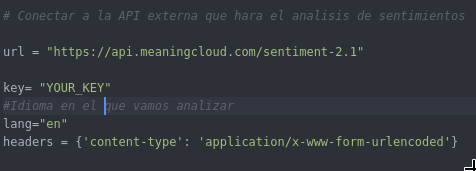
\includegraphics[scale=.35]{imagenes/key-analisis.png}
	\caption{Declaración de variables necesarias para la API de MeaningCloud}
	\label{fig:key-analisis}
\end{figure}




El código recorrerá toda la colección \textit{tweets} de la base de datos MongoDB, mandando únicamente el texto de los tweets a MeaningCloud, pues es la información que deberá ser analizada. Extraemos la información de utilidad de la respuesta y la almacenamos en diferentes variables. Dichas variables son:

\begin{itemize}
	\item \textbf{Confidence:} Es el valor de fiabilidad del análisis. MeaningCloud asigna un valor de 0-100, siendo 100 lo más fiable posible a la calidad de su análisis. Sólo cogeremos los resultados de los análisis aceptables, es decir, que tengan un valor superior a 90.
	\item \textbf{Score\_tag:} Posiblemente la variable más importante del análisis. Puesto que clasificará entre muy positivo y muy negativo el tono emocional del texto analizado. Su rango de polaridad es: 
	\begin{itemize}
		\item P+: Muy positivo
		\item P: Positivo
		\item NEU: Neutral
		\item N: Negativo
		\item N+: Muy negativo
		\item NONE: Ninguno, no se le ha detectado ningún tono emocional al texto.
	\end{itemize}
	\item \textbf{Agreement:} Si hay más de un sentimiento detectado en el texto, si estos sentimientos tienen el mismo tono emocional o no. 
	\item \textbf{Subjectivity:} Subjetividad. Como su nombre indica, indica si el texto era objetivo o subjetivo.
	\item \textbf{Irony:} Indica si el texto era irónico o no. Por experiencia al usarlo esta variable será ignorada puesto que tras comprobarlo su tasa de acierto es muy baja o nula. 
	\item \textbf{Sentimented\_Entity\_List:} Lista de entidades en el texto de las cuales tienen una polaridad, es decir, generan un tono emocional en el autor. Nombres de compañías de servicio, ciudades, países, nombres de usuario. Reconoce un gran rango de entidades. 
	\item \textbf{Sentimented\_Concept\_List:} Lista de conceptos en el texto los cuales tienen polaridad concreta. 
\end{itemize}

Finalmente, tras su análisis. Si la confianza en el análisis está en un rando aceptable, almacenamos los datos en un fichero CSV y en la nueva colección \textit{concepts} que hemos creado dentro de la misma base de datos. Es importante notar que este análisis no admite la introducción de emojis, por lo que los tweets que contengan emojis serán devueltos con un mensaje de Error, el cual no interrumpirá el análisis y simplemente seguirá analizando el resto de la base de datos. 


\begin{figure}[H]
	\centering
	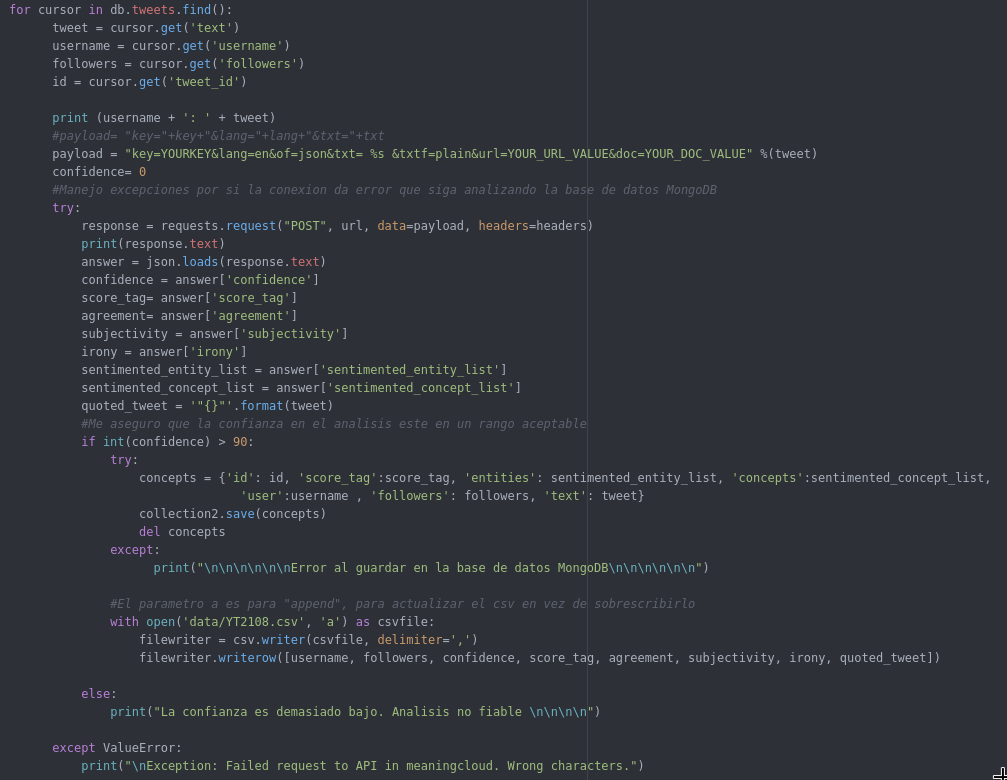
\includegraphics[scale=.35]{imagenes/bucle-analisis.png}
	\caption{Bucle para recorrer la BD de Mongo y analizarla}
	\label{fig:bucle-analisis}
\end{figure}

NOTA: Existe otro script llamado \textbf{analisis-desde-nombre}, el cual es casi idéntico al anteriormente descrito cuya única diferencia es que podemos analizar la base de datos desde un usuario determinado. Por lo que si hay un error, como puede ser una perdida de conexión, será tan trivial como abrir el fichero CSV, buscar el nombre del último usuario añadido al fichero y escribir dicho nombre en la comprobación del script para continuar la búsqueda sin repetir tweets y sin perder información. 



\subsection{WordCloud}

Se ha diseñado un script, que recorrerá todas las palabras de todos los tweets del fichero CSV. Pudiendo con esta información realizar un WordCloud donde aparezcan las palabras más usadas entre todos los tweets. Para ello se hará uso de unas librerías matemáticas de uso científico. Las más importantes serán: 

\begin{itemize}
	\item NumPy: Extensión de python específica para darle mayor soporte para vectores y matrices. Constituye una librería de funciones matemáticas de alto nivel.
	\item Pandas: Estrechamente relacionada con la bibliotea NumPy está orientada a la manipulación y análisis de datos. 	
	\item Matplotlib: biblioteca para la generación de gráficos a partir de datos contenidos en listas o arrays, relacionada también con la extensión NumPy. Diseñada para ser similar a la utilizada en MATLAB
	\item PIL: Python Imaging Lybrary, es una biblioteca que añade soporte para abrir, manipular y almacenar muchos formatos de imagen distintos. 
	
\end{itemize}


\begin{figure}[H]
	\centering
	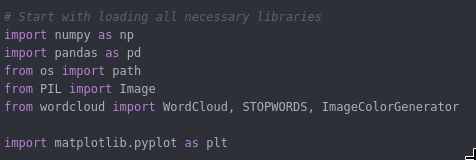
\includegraphics[scale=.5]{imagenes/include-words.png}
	\caption{Librerías utilizadas en el script de WordCloud}
	\label{fig:include-words}
\end{figure}


El código extrairá la información del fichero CSV deseado con la función \textit{read\_csv()} de la librería Pandas. Como información añadida mostrará por pantalla cuantos tweets hay de cada polaridad, desde muy positivo a muy negativo, también hará un recuento de las palabras que haya en el total de todos los tweets juntos. Los cuales se juntarán todos en una sola variable denominada text gracias a un bucle y la facilidad de manipulación de datos que ofrece Pandas.
 
 Finalmente para este fragmento, se le introduce una imagen previamente seleccionada, la cual hará de plantilla para la posterior generación del WordCloud, es decir, en vez de usar la forma en la que aparece por defecto, usará la forma y colores de la imagen que se le introduzca. Esta imagen deberá estar en formato RPG pues gracias a Numpy se generará una máscara con la imagen transformada en un array de datos. La función array de Numpy transforma la imagen en un vector de datos comprendidos en un rango de 0-255 que contendrán la información de la imagen en un formato que el algoritmo pueda procesar.

\begin{figure}[H]
	\centering
	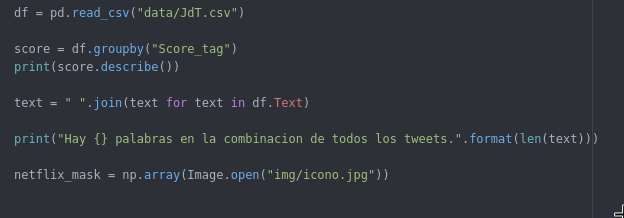
\includegraphics[scale=.5]{imagenes/lectura-imagen-words.png}
	\caption{Lectura de la imagen de plantilla y unificación de todos los tweets en una única variable}
	\label{fig:include-words}
\end{figure}


Una opción para la creación del WordCloud es la asignación de Stopwords, los cuales serán palabras que no se mostrarán en el fichero que se cree. Puesto que hay palabras que debido al formato de los tweets son propensas a aparecer mucho, podemos quitarlas para obtener un WordCloud más satisfactorio. Por ejemplo, si tengo una base de datos acerca de Netflix, es asumible que todos los tweets contendrán la palabra Netflix, sabiendo esto incluimos a Netflix entre los Stopwords para que en el fichero generado veamos las palabras más usadas para hablar de la plataforma, no la plataforma en sí. 

\begin{figure}[H]
	\centering
	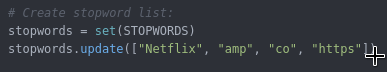
\includegraphics[scale=.7]{imagenes/stopword.png}
	\caption{Adición de Stopwords al WordCloud}
	\label{fig:stopwords}
\end{figure}


Ahora queda la generación del WordCloud en sí. Llamando a la función \textit{WordCloud()} en la que introducimos los parámetros deseados, entre los que destacan el número máximo de palabras que generaremos, la máscara que indicará la forma que debe tomar el wordcloud en sí, los stopwords que se han añadido con prioridad, el grosor de los bordes, de tenerlos, de la plantilla y el color de dichos bordes. Con la función \textit{ImageColorGenerator()} a la cual se le añade como parámetro la máscara generada con NumPy, indicará qué colores darle a las palabras al pintar la figura. Para finalizar, con las funcionalidades de Matplotlib se pintará la imagen, habiendo que indicarle el tamaño de la figura resultante y pasarle la variable de wordcloud que contiene las palabras y por parámetro el color que deseamos que tengan dichas palabras para respetar el formato original. Guarda la figura con el nombre y formato deseado y la muestra por pantalla. 

\begin{figure}[H]
	\centering
	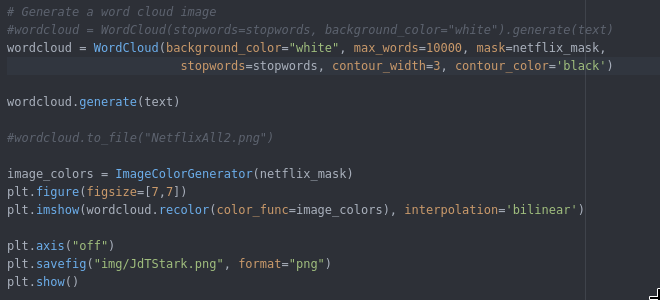
\includegraphics[scale=.5]{imagenes/generar-words.png}
	\caption{Generación de la imagen del WordCloud}
	\label{fig:generacion-words}
\end{figure}












